\bexo
Tracer sur la même figure
\begin{itemize}
	\item $t\mapsto \ln(t)$
	\item $t\mapsto \ln(2t)$
	\item $t\mapsto \ln(2t-1)$
\end{itemize}
	
	\begin{center}
	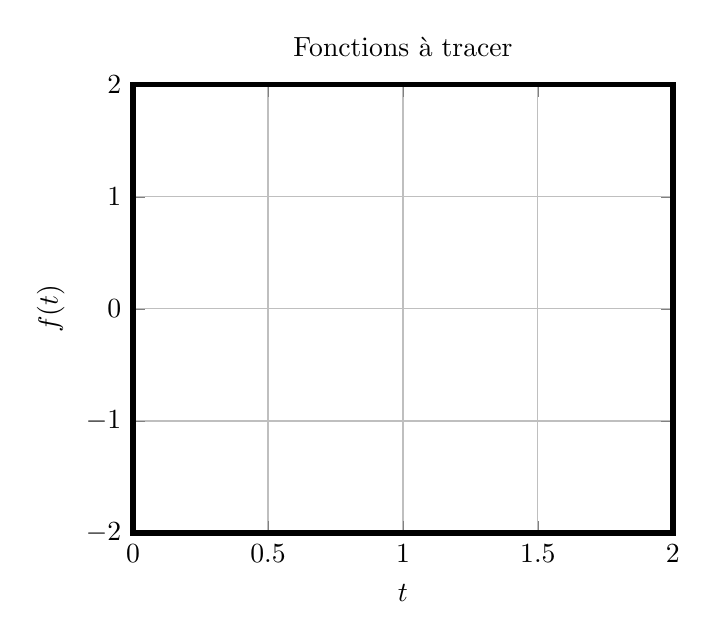
\begin{tikzpicture}
	  \begin{axis}[line width=2pt,       legend columns=-1,
   title=Fonctions à tracer,
   xlabel={$t$},
   ylabel={$f(t)$}, xmin=0,
xmax=2,
ymin=-2, 
ymax=2,
	  legend to name=named , grid=major]
	%	\addplot[white] expression[domain=-pi:pi,samples=500]{4*cos(180*x/pi)};
	  \end{axis}
	\end{tikzpicture}
\ref{named}
\end{center}


	

\eexo
\solution{
Les graphes des fonctions sont:\\

	\begin{center}
	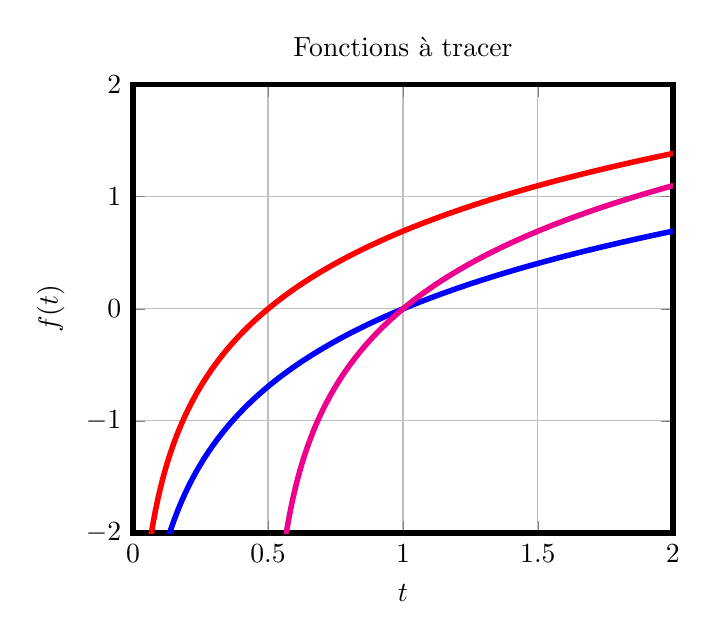
\begin{tikzpicture}
	  \begin{axis}[line width=2pt,       legend columns=-1,
   title=Fonctions à tracer,
   xlabel={$t$},
   ylabel={$f(t)$}, xmin=0,
xmax=2,
ymin=-2, 
ymax=2,
legend entries={$\ln(t)$,$\ln(2t)$,$\ln(2t-1)$},
	  legend to name=named , grid=major]
		\addplot[blue] expression[domain=0.0001:pi,samples=500]{ln(x)};
		\addplot[red] expression[domain=0.0001:pi,samples=500]{ln(2*x)};
		\addplot[magenta] expression[domain=0.5001:pi,samples=500]{ln(2*x-1)};
\end{axis}
	\end{tikzpicture}
		  \ref{named}
\end{center}


}